\chapter{An Approach to Resource-centric Organizational Modeling}
\label{chap:approach}

This section describes in detail about the technical approach that has been taken to solve the problem mentioned in problem statement section of Chapter \ref{chap:introduction}. This chapter also provides an outline of the design, the methodology and overall structure of the approach. The first section of this chapter provides an overview of modeling process approach. The second section  provides a brief description about the frameworks and libraries used. The third section discusses in detail about the \textit{top-down approach}, which has been used to realize the resource-centric organizational modeling. The fourth section discusses the design methodology followed to realist this approach of developing a descriptive modeling web based editor. The final section discusses in detail about the relationship between each entity types of this approach. The main contribution of this approach is to explain the concepts in a concrete way, whose abstract concepts are discussed in earlier chapters.

%%%%%%%%%%%%%%%%%%%%%%%%%%%%%%%%%%%%%%%%%%%%%%%%%%%%%%%%%%%%%%%%%%%%%%%%%
\section{Overview of the Modeling Process}
\label{sec:overviewmodelingprocess}
%%%%%%%%%%%%%%%%%%%%%%%%%%%%%%%%%%%%%%%%%%%%%%%%%%%%%%%%%%%%%%%%%%%%%%%%%
The main focus of this approach is to develop a web-based editor which can be used by business experts to model the informal processes. Also in this thesis work, the scope of modeling is limited only to the descriptive type of modeling. As we mentioned before, the resource definitions required for the editor is made available from the first phase P1 of the InProXec approach. Business experts develop descriptive models through the editor using these resources to achieve main intention that contains sub-intentions, strategies etc. The reason for following descriptive modeling approach is due to the fact that models reusable descriptive data and these stored models provides means of execution for the phases P3 and P4 of InProXec. The model provides necessary concepts and relations for modeling the core elements of resource centric organizational modeling. Resources are abstract description which are made concrete during initialization of an instance. There are also resource specific views based on the participating resources' role. For example, based on the privilege provided to a participant he can view/edit/own/follow the instances. Initializing resource-centric  models requires \textit{acquiring} and engaging interrelated resources which is explained in detail in the following sections of this chapter. 

%%%%%%%%%%%%%%%%%%%%%%%%%%%%%%%%%%%%%%%%%%%%%%%%%%%%%%%%%%%%%%%%%%%%%%%%%
\section{Technologies and Frameworks}
\label{subsec:specifications}
%%%%%%%%%%%%%%%%%%%%%%%%%%%%%%%%%%%%%%%%%%%%%%%%%%%%%%%%%%%%%%%%%%%%%%%%%
In order to realize the web-based editor of Intention-centric Organizational Modeling, a formal inquiry has been done to choose suitable technologies and frameworks required. The below specifications were finalized and \textit{client-side scripting}\footnote{https://en.wikipedia.org/wiki/Client-side\_scripting} has been chosen due to the fact that our developed editor is web-based. 

\begin{enumerate}   
	\item \textit{Clojure}\footnote{https://clojure.org/} as the programming language
	\item \textit{IntelliJIDEA}\footnote{https://www.jetbrains.com/idea/} as the development environment
	\item \textit{MVC}  as the architecture pattern
	\item \textit{Re-frame}\footnote{https://github.com/Day8/re-frame} as the pattern for writing SPAs in ClojureScript, using Reagent	
\end{enumerate}

Other than the above listed frameworks and technologies, frameworks like \textit{react-bootstrap}\footnote{https://react-bootstrap.github.io/}, jquery\footnote{https://jquery.com/} were also used to provide more optimal view of the editor. \textit{Clojure} is a dynamic, general-purpose programming language, combining the approachability and interactive development of a scripting language with an efficient and robust infrastructure for multithreaded programming. \textit{ClojureScript}\footnote{http://clojure.org/about/clojurescript} is a compiler for Clojure that targets JavaScript which has been designed to emit JavaScript code. In our implementation, we have used both Clojure and Clojurescript. We also used \textit{Reagent}\footnote{http://reagent-project.github.io/} which provides a minimalistic interface between ClojureScript and React\footnote{https://facebook.github.io/react/}. A \textit{Re-frame}\footnote{https://github.com/Day8/re-frame} is a pattern for writing applications in ClojureScript, using Reagent.

%%%%%%%%%%%%%%%%%%%%%%%%%%%%%%%%%%%%%%%%%%%%%%%%%%%%%%%%%%%%%%%%%%%%%%%%%
\subsection{MVC Architecture}
\label{subsec:mvcarch}
%%%%%%%%%%%%%%%%%%%%%%%%%%%%%%%%%%%%%%%%%%%%%%%%%%%%%%%%%%%%%%%%%%%%%%%%%
 The architecture of the developed user interface of the editor is based on the \textbf{Model-View-Control (MVC)} design pattern. The MVC paradigm allows to separate business logic from the code that controls presentation and event handling \cite{Oracle2016}.Each entity view in the web page is made up of combination of at least on Model and View, and one or more Controls. The functionalities of individual files which acts an Model, View and Controller has been shown in the Figure \ref{fig:mvc_arch}

\begin{figure}
	\centering
	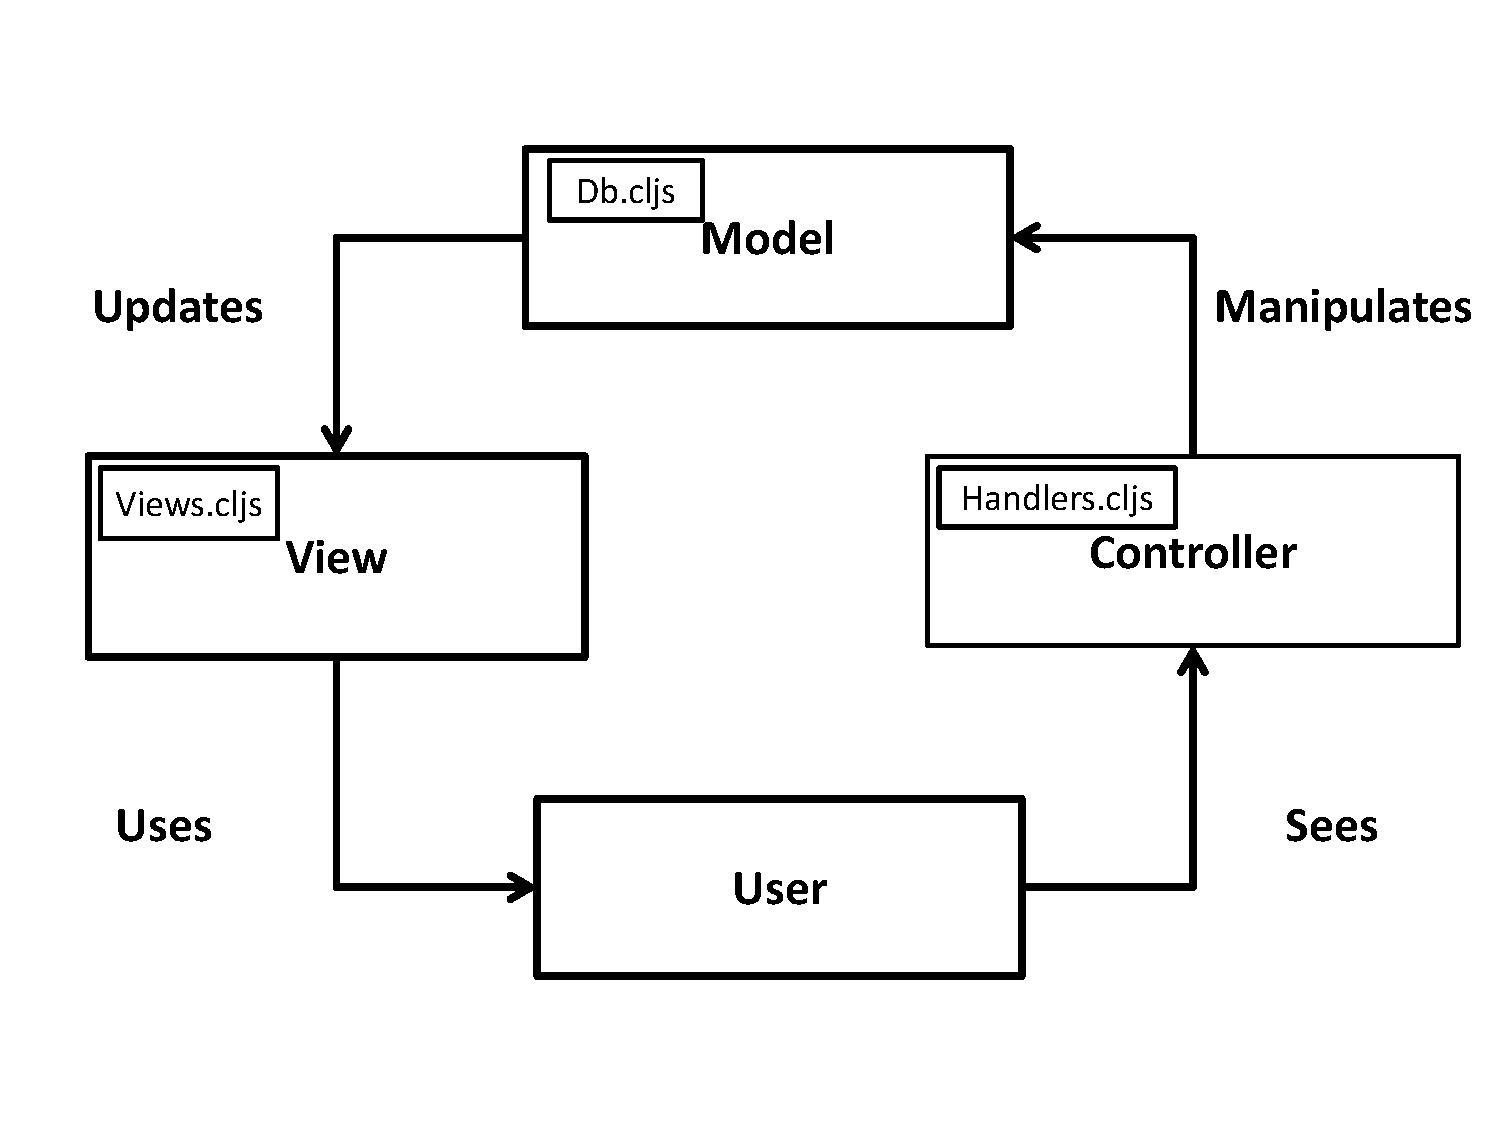
\includegraphics [width= 0.75\textwidth]{mvc_arch.pdf}
	\caption{MVC architecture components}
	\label{fig:mvc_arch}
\end{figure}

\textit{Model} artifact stores the required data structure for web-editor. In the developed model artifact, the four main types of data stored inside the artifact are intentions, strategies, capabilities and informal process instances. 

\textit{View} artifact contains HTML elements and HTML constructs that describe the way of displaying the data from Model to the user. Most of the common functionalities that render user interface components are re-used. 

\textit{Control} artifact contains the handler functions which can only change the model. Even the initial values of the model are put inside the control. This artifact has functions causes default database to change, which then causes a re-render of view and then the user sees new view.
	
Apart from the above artifacts, there is another important artifact that registers subscription functions i.e., query layer of the data. As view components never source data directly from default model, we use \textit{subscription} functions. Subscription  functions returns a value that changes over time i.e based on a user events.

%%%%%%%%%%%%%%%%%%%%%%%%%%%%%%%%%%%%%%%%%%%%%%%%%%%%%%%%%%%%%%%%%%%%%%%%%
\subsubsection{Example: Component using MVC Pattern }
%%%%%%%%%%%%%%%%%%%%%%%%%%%%%%%%%%%%%%%%%%%%%%%%%%%%%%%%%%%%%%%%%%%%%%%%%
 The Figure \ref{fig:mvc_arch} below shows the simplifed version of how the components interact with each other using the Model-View-Control (MVC) pattern, for the functionality of adding new entity data. This functionality is same for all the types such as intentions, strategies, capabilities and informal processes and below is the detailed explanation of each interaction.
 
 \begin{figure}
 	\centering
 	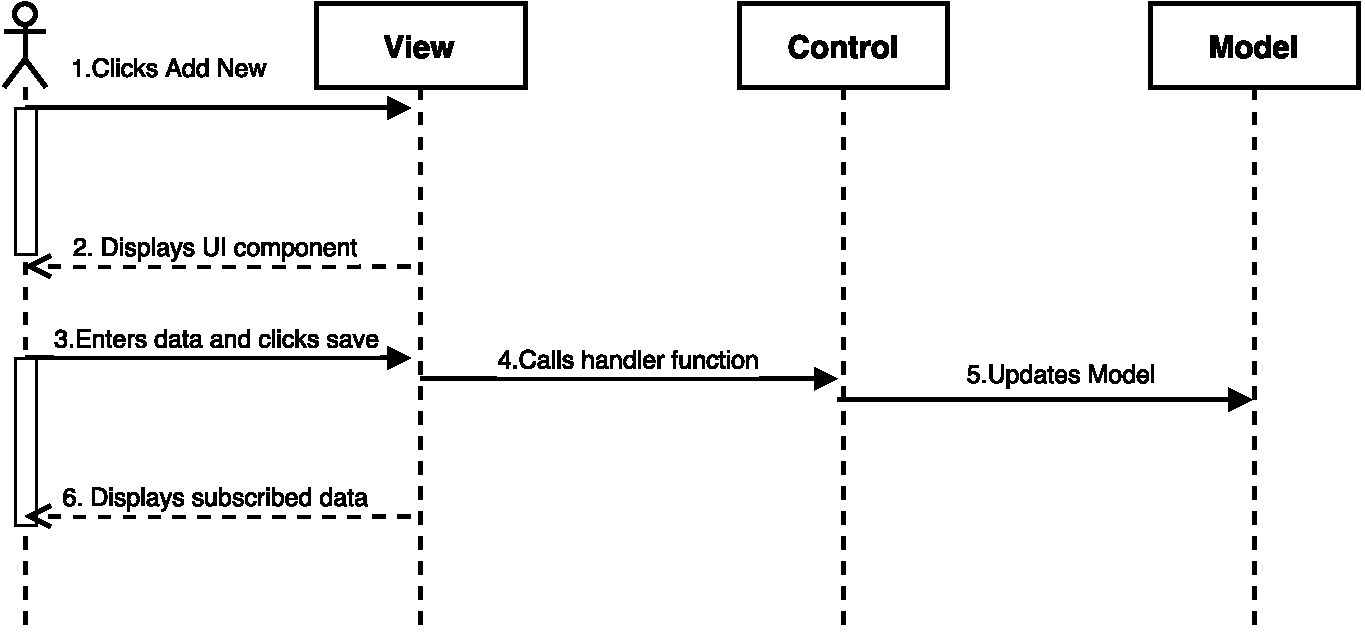
\includegraphics [width= \textwidth]{mvc_pattern.pdf}
 	\caption{MVC Pattern of adding new entity}
 	\label{fig:mvc_pattern}
 \end{figure}

\begin{enumerate}
	\item User clicks the tab \textbf{Add New} button in the developed editor.
	\item In response to the user click, the view displays the respective user interface component for entering the new entity data details.
	\item User enters the required basic details for adding new entity data and clicks save button.
	\item The view dispatches the data to control, which can only modify the model.
	\item Control inserts/updates data into the model.
	\item View displays the updated model as it has been subscribed to the model.
\end{enumerate}

%%%%%%%%%%%%%%%%%%%%%%%%%%%%%%%%%%%%%%%%%%%%%%%%%%%%%%%%%%%%%%%%%%%%%%%%%
\section{A Top-Down Modeling Approach}
\label{sec:topdownapproach}
%%%%%%%%%%%%%%%%%%%%%%%%%%%%%%%%%%%%%%%%%%%%%%%%%%%%%%%%%%%%%%%%%%%%%%%%%
Intentions are defined hierarchically, intentions can contain and extend intentions which are called as sub-intentions. Intentions can contradict to itself as well. Intentions are associated with strategies, thus intentions can be realized through strategies. Strategies are associated with capabilities. These capabilities are of two types \textit{functional capabilities} and \textit{cross functional capabilities}. Functional capabilities are associated with resources and cross functional capabilities are associated with functional capabilities. Each informal process model is a strategy that has capabilities, strategies, resources that are created out of capabilities and intentions. In the Figure \ref{fig:topdownapproach}, it has been shown that how this modeling approach starts modeling from top level of the hierarchy and does modeling until the lower level is reached. 

\begin{figure}
	\centering
	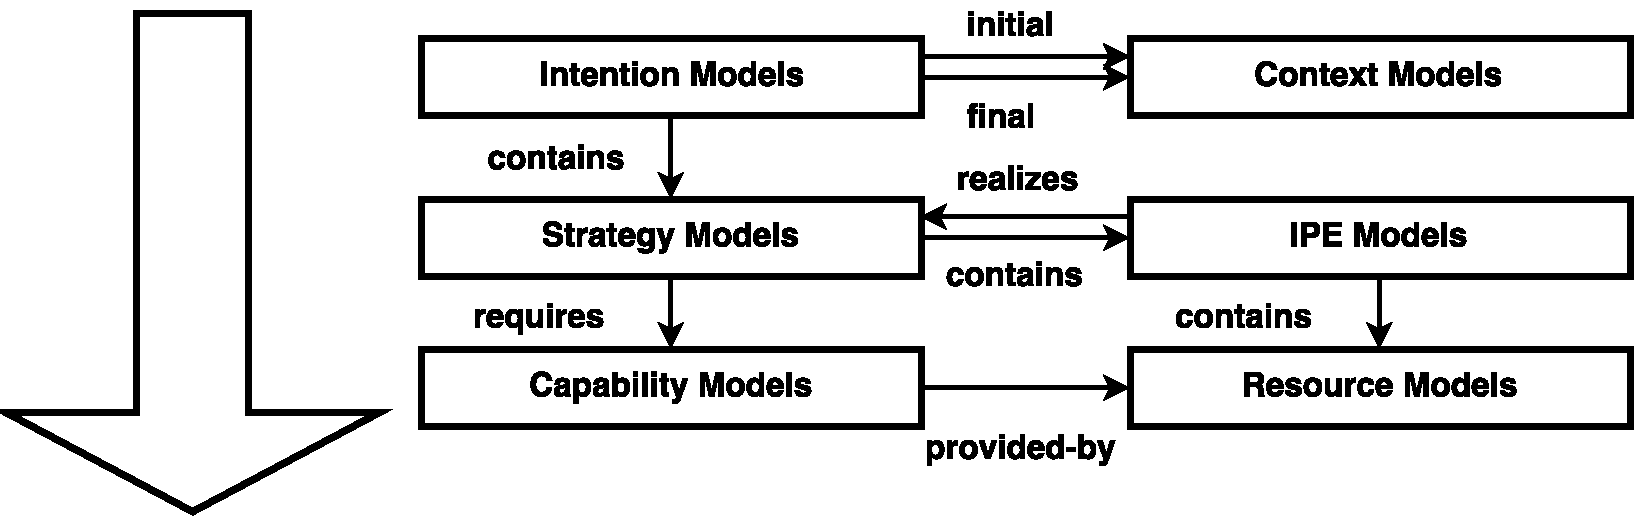
\includegraphics[width=\textwidth]{TopDownApproach.pdf}
	\caption{Top Down Modeling Approach}
	\label{fig:topdownapproach}
\end{figure}

Bider et al \cite{bider2005strategy} propose a strategy-driven modeling approach of processes. Processes are defined based on the goals and refinement continues until meaningful operation level is reached. Consequently, created models are easily changeable as they are decoupled from their operational terms. Such declarative approaches provide more flexibility and enable easier change of the business process models \cite{Sungur2016}. As we mentioned before, the modeling approach in our context is descriptive modeling approach which starts from the top level and refines modeling until the bottom level is reached. 



%%%%%%%%%%%%%%%%%%%%%%%%%%%%%%%%%%%%%%%%%%%%%%%%%%%%%%%%%%%%%%%%%%%%%%%%%
\section{Design Methodology}
\label{sec:designmethodology}
%%%%%%%%%%%%%%%%%%%%%%%%%%%%%%%%%%%%%%%%%%%%%%%%%%%%%%%%%%%%%%%%%%%%%%%%%
When designing the user interface components and functionalities required to develop the tool, most of the similar functionalities are 
designed as common functionalities and re-used. This reduces the unnecessary functional redundancies and overhead. The common functionality methodology are implemented for both model functions and view functions.  Some of important methodologies followed with respect to user interface components design are 1. multiple items to be selected from multiple items are displayed as  \textit{list} 2. selecting single item from multiple items are displayed as drop down. For example, to select multiple strategies from a list of strategies, available strategies are displayed as a list from which the user can select desired number of strategies. Another important methodology followed during user interface design is, for every entity their properties should be displayed only under their respective properties tab. For example in the figure \ref{fig:samplescreen}, the basic properties such as name, target namespace and process type of an informal process model should be displayed only under the respective basic properties tab. This methodology is followed uniformly throughout the design of all the entity types such as intention definitions, strategy definitions, capability defintions, context definitions, instance definitions and informal process definitions and for all of their property types. 
All data are stored only under the data artifact. This applies to the labels and text fields of all user interface elements and this data can be updated only through the handler function. Through \textit{settings} option, the user also has option to add new namespace and intention relation type. 

\begin{figure}
	\centering
	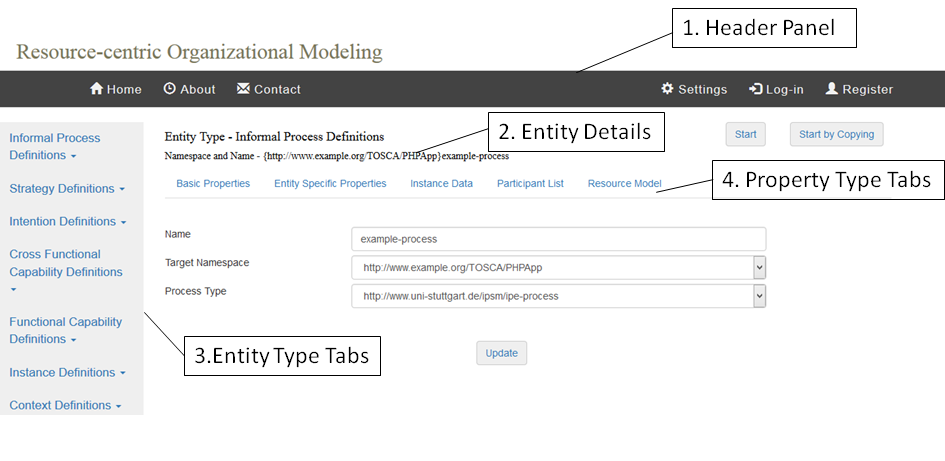
\includegraphics[width=\textwidth,angle=0]{samplescreen.png}
	\caption{User Interface Design of the Editor}
	\label{fig:samplescreen}
\end{figure}

The research objectives mentioned in Chapter \ref{chap:introduction} are also met during the development of the editor. The validity of the research objectives are discussed in Chapter \ref{chap:casestudy} using the motivating scenario discussed in Chapter \ref{chap:motivatingScenario}.

\textit{Organizational intentions transparency} (R1): In the current functioning system, users are stored in database artifact and these users can login through their valid credentials. 

\textit{Organizational intention resource-based cost estimation} (R2): Intentions are associated with strategies, which are associated with capabilities and hence with resources. Cost is calculated in a recursive manner. For example, consider we need to calculate cost of an instance whose entity type is intention. To calculate the cost we go recursively to the lower levels starting from the required level. Since our instance is of type intention, we start iterating through every associated strategy, and for each associated strategy, we iterate through their instance descriptors as well. In case the cost of an instance descriptor of a strategy has not been specified, we specify it by calculating the cost of instance descriptors of associated informal process definitions. For informal process definitions, we use the cost resource definitions. This ends the recursion and returns the total sum as the cost of an instance of type intention

\textit{Organizational intention achievability estimation} (R3): Similar to resource-based cost estimation for an intention, the achievability of an intention also depends on its instance state. For example, if an instance of type intention is associated with a strategy which also has an instance that is completed. Then the total number instances remaining to be completed to achieve an intention is calculated as one out two instances. 

\textit{Intention oriented working style} (R4): The users can login and create intention models, strategy models, informal process models etc., through the developed editor. 

\textit{Participative organizational modeling} (R5): Each entity type that can be acquired or instantiated has list of participants with their corresponding privileges. 

\textit{Re-use of organizational knowledge} (R6): The descriptive information about each models can be stored and re-used for next enactments. 
 
%%%%%%%%%%%%%%%%%%%%%%%%%%%%%%%%%%%%%%%%%%%%%%%%%%%%%%%%%%%%%%%%%%%%%%%%%
\section{Characteristics of the Entity Types}
\label{sec:enttyperelation}
%%%%%%%%%%%%%%%%%%%%%%%%%%%%%%%%%%%%%%%%%%%%%%%%%%%%%%%%%%%%%%%%%%%%%%%%%
The entity types are modeled as descriptive informations, this is because models can be initialized and can be made runnable elements which are required for subsequent phases such as P3 and P4 of InProXec. An IPE model describes the main intention that reflects the informal process' main goal. Each intention may be refined into sub-intentions. The IPE model's initial context specified the triggers that signal when model's corresponding resources should be initialized and subsequently work towards the informal process' main intention\cite{Sungur2015a}. The final context specifies conditions for determining the processes' main intention as successfully achieved. 



%%%%%%%%%%%%%%%%%%%%%%%%%%%%%%%%%%%%%%%%%%%%%%%%%%%%%%%%%%%%%%%%%%%%%%%%%
\subsection{Context Intention Relationship}
\label{sec:ctxintrel}
%%%%%%%%%%%%%%%%%%%%%%%%%%%%%%%%%%%%%%%%%%%%%%%%%%%%%%%%%%%%%%%%%%%%%%%%%
Intentions connect initial context definitions with final context definitions Figure \footnote{C Timurhan Sungur, An approach to supporting and automating informal processes, May 2015}.


\begin{figure}
	\centering
	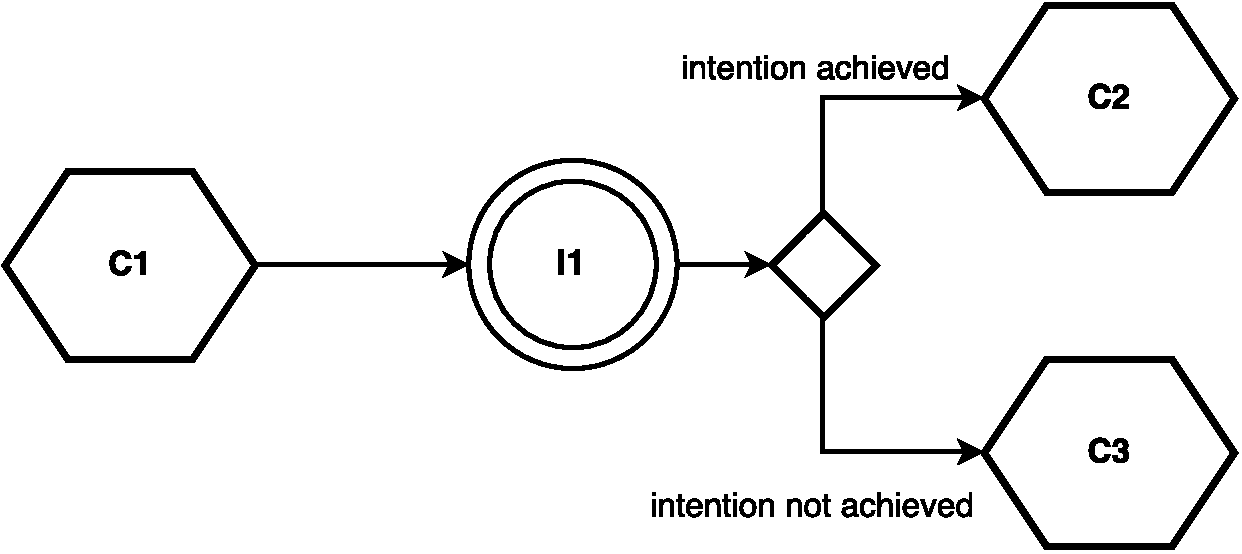
\includegraphics[width=\textwidth,angle=0]{orgIntContext.pdf}
	\caption{Context Intention Relationship}
	\label{fig:orgIntentions}
\end{figure}

%%%%%%%%%%%%%%%%%%%%%%%%%%%%%%%%%%%%%%%%%%%%%%%%%%%%%%%%%%%%%%%%%%%%%%%%%
\subsection{Capabilities Resource Relationship}
\label{sec:capIntRel}
%%%%%%%%%%%%%%%%%%%%%%%%%%%%%%%%%%%%%%%%%%%%%%%%%%%%%%%%%%%%%%%%%%%%%%%%%
Each organizational capability must be provided by a resource in the organization. Resource models are optional to make precise definitions of resources needed. The relationship between organizational capabilities and organizational intentions has been provided in the Figure 
 
\begin{figure}
	\centering
	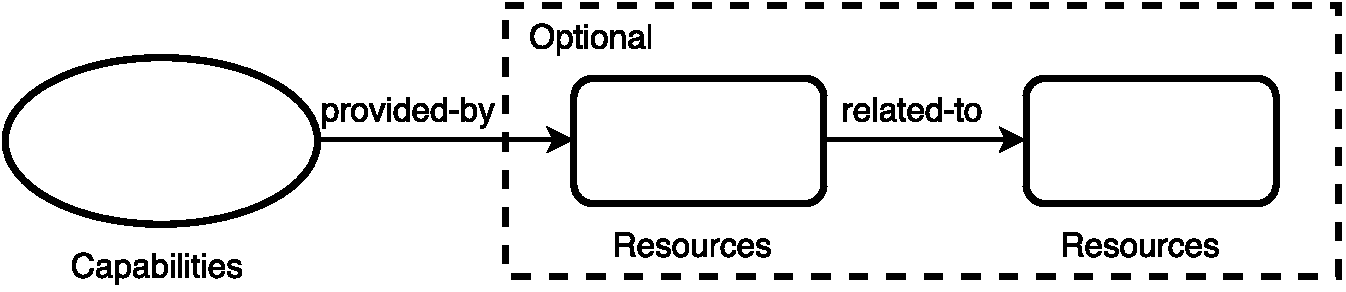
\includegraphics[width=\textwidth,angle=0]{capabilitiesResources.pdf}
	\caption{Capabilities Resources Relationship}
	\label{fig:capabilitiesresources}
\end{figure}

Each \textit{intention} can require certain \textit{capabilities} which are provided by \textit{organizational resources}. 
As a result each informal process model is a strategy and will have cross-functional capabilities, resources (which will be created out of capabilities), a goal that the specific strategy.





%%%%%%%%%%%%%%%%%%%%%%%%%%%%%%%%%%%%%%%%%%%%%%%%%%%%%%%%%%%%%%%%%%%%%%%%%
\subsection{Acquirable Entity Types}
\label{sec:acquirableentities}
%%%%%%%%%%%%%%%%%%%%%%%%%%%%%%%%%%%%%%%%%%%%%%%%%%%%%%%%%%%%%%%%%%%%%%%%%
Final state of the model instance is saved Figure \ref{fig:acquirableentities}.

\begin{figure}
	\centering
	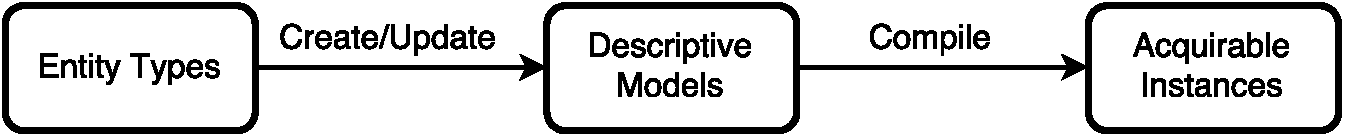
\includegraphics[width=\textwidth,angle=0]{AcquirableEntities.pdf}
	\caption{Acquirable Instances}
	\label{fig:acquirableentities}
\end{figure}



